\PassOptionsToPackage{unicode=true}{hyperref} % options for packages loaded elsewhere
\PassOptionsToPackage{hyphens}{url}
%
\documentclass[
]{article}
\usepackage{lmodern}
\usepackage{amssymb,amsmath}
\usepackage{ifxetex,ifluatex}
\ifnum 0\ifxetex 1\fi\ifluatex 1\fi=0 % if pdftex
  \usepackage[T1]{fontenc}
  \usepackage[utf8]{inputenc}
  \usepackage{textcomp} % provides euro and other symbols
\else % if luatex or xelatex
  \usepackage{unicode-math}
  \defaultfontfeatures{Scale=MatchLowercase}
  \defaultfontfeatures[\rmfamily]{Ligatures=TeX,Scale=1}
\fi
% use upquote if available, for straight quotes in verbatim environments
\IfFileExists{upquote.sty}{\usepackage{upquote}}{}
\IfFileExists{microtype.sty}{% use microtype if available
  \usepackage[]{microtype}
  \UseMicrotypeSet[protrusion]{basicmath} % disable protrusion for tt fonts
}{}
\makeatletter
\@ifundefined{KOMAClassName}{% if non-KOMA class
  \IfFileExists{parskip.sty}{%
    \usepackage{parskip}
  }{% else
    \setlength{\parindent}{0pt}
    \setlength{\parskip}{6pt plus 2pt minus 1pt}}
}{% if KOMA class
  \KOMAoptions{parskip=half}}
\makeatother
\usepackage{xcolor}
\IfFileExists{xurl.sty}{\usepackage{xurl}}{} % add URL line breaks if available
\IfFileExists{bookmark.sty}{\usepackage{bookmark}}{\usepackage{hyperref}}
\hypersetup{
  pdftitle={Oversikt over PROM-skjema},
  pdfauthor={Rapporteket},
  pdfborder={0 0 0},
  breaklinks=true}
\urlstyle{same}  % don't use monospace font for urls
\usepackage{graphicx,grffile}
\makeatletter
\def\maxwidth{\ifdim\Gin@nat@width>\linewidth\linewidth\else\Gin@nat@width\fi}
\def\maxheight{\ifdim\Gin@nat@height>\textheight\textheight\else\Gin@nat@height\fi}
\makeatother
% Scale images if necessary, so that they will not overflow the page
% margins by default, and it is still possible to overwrite the defaults
% using explicit options in \includegraphics[width, height, ...]{}
\setkeys{Gin}{width=\maxwidth,height=\maxheight,keepaspectratio}
\setlength{\emergencystretch}{3em}  % prevent overfull lines
\providecommand{\tightlist}{%
  \setlength{\itemsep}{0pt}\setlength{\parskip}{0pt}}
\setcounter{secnumdepth}{-2}
% Redefines (sub)paragraphs to behave more like sections
\ifx\paragraph\undefined\else
  \let\oldparagraph\paragraph
  \renewcommand{\paragraph}[1]{\oldparagraph{#1}\mbox{}}
\fi
\ifx\subparagraph\undefined\else
  \let\oldsubparagraph\subparagraph
  \renewcommand{\subparagraph}[1]{\oldsubparagraph{#1}\mbox{}}
\fi

% set default figure placement to htbp
\makeatletter
\def\fps@figure{htbp}
\makeatother

%\documentclass{article}
\usepackage{xcolor}
\usepackage{sectsty}
\usepackage{marginnote}
\usepackage[norsk]{babel}
\usepackage[left=5cm,%
            right=2cm,%
            top=2.25cm,%
            bottom=2.25cm,%
            headheight=12pt,%
            letterpaper,%
            reversemarginpar,%
            marginparwidth=3.25cm,%
            marginparsep=2em%
            ]{geometry}

% \usepackage[utf8x]{inputenc}
% \usepackage{authblk}
% \usepackage{longtable}
% \usepackage{microtype}
% \usepackage{multicol}
% \usepackage{wasysym}
% \usepackage[raggedright]{titlesec}
% \usepackage[breaklinks]{hyperref}
% \usepackage[color]{changebar}

% Oppsett av fonter
\usepackage[defaultsans]{lato}
\renewcommand{\familydefault}{\sfdefault}

\usepackage[font={rm},labelfont={bf,sf},%
            labelsep=period,%
            skip=4pt,tableposition=top,%
            singlelinecheck=false,justification=centering]{caption}

% Oppsett hode, kne og tå
\usepackage{fancyhdr}  % custom headers/footers
\usepackage{lastpage}  % Number of pages in the document
\pagestyle{fancy}      % Enables the custom headers/footers

% Headers
\makeatletter
\renewcommand{\sectionmark}[1]{\markright{#1}}
\renewcommand{\subsectionmark}[1]{\markright{#1}}
\lhead{\small\sffamily\bfseries\@author}%
\chead{}%
\rhead{\small\sffamily\bfseries\nouppercase{\rightmark}}%
% Footers
\lfoot{\small\sffamily\bfseries\@title}%
\cfoot{}%
\rfoot{\small\sffamily\bfseries\thepage/\pageref{LastPage}}%
\renewcommand{\headrulewidth}{0.1pt}%
\renewcommand{\footrulewidth}{0.1pt}%
\makeatother


% Oppsett tittelside
\makeatletter
\let\authblk@author\author
\let\oldaffil\affil

\usepackage[absolute]{textpos}
\renewcommand{\@maketitle}{%
    \def\@makefnmark{}%
    \begin{textblock*}{\marginparwidth}[1,0]%
      (\dimexpr\Gm@lmargin-\marginparsep,\Gm@tmargin)
      \raggedleft\footnotesize%
      
\includegraphics[width=\hsize]{logo_smerte}%
      \raggedleft\footnotesize%
      {\\ SMERTEREGISTERET er et nasjonalt kvalitetsregister som kvalitesforbedring av smertebehansling som formål. Bla, bla, bla...\par}
      
\includegraphics[width=\hsize]{logo}%
      {\\ RAPPORTEKET er en analysetjenste som tilbyr interaktiv undersøkelse av rådata, rutinemessig utsending av rapporter og visualisering av resultater. Tjenesten utvikles og vedlikeholdes av Nasjonalt servicemiljø for medisinske kvalitetsregistre ved Senter for Klinisk Dokumentasjon og Evaluering (SKDE) og arbeidet finansieres av Helse- og omsorgsdepartementet.}%
    \end{textblock*}
    %
    \begin{textblock*}{\marginparwidth}[1,1]%
      (\dimexpr\Gm@lmargin-\marginparsep,\dimexpr\paperheight-\Gm@bmargin)
      \raggedleft\footnotesize\itshape%
      {\large\rmfamily\upshape\bfseries Om rapporten\par}%
      {\textbf{Bestilt av}\\\@author\par}%
      {\textbf{Produsert av}\\ Rapporteket\par}%
      {\textbf{Dato}\\ dato\par}%
      {\textbf{Tid}\\ tid\par}%
      {\textbf{Fingeravtrykk}\\ fingeravtrykk\par}%
    \end{textblock*}

    {\raggedright\sffamily\bfseries\fontsize{20}{25}\selectfont\@title\par}%
    \vskip10pt
    {\raggedright\@author\par}
    \vskip18pt%
}
\apptocmd{\maketitle}{\thispagestyle{empty}}{}{}
\makeatother
%-----------------------------------------------




% Bruk hf-rager på nivå 1 og 2 overskrifter
\definecolor{hfmork}{RGB}{0,82,155}
\definecolor{hflys}{RGB}{104,174,224}
\subsectionfont{\color{hflys}}
\sectionfont{\color{hfmork}}

\usepackage[explicit]{titlesec}
\titleformat{\section}
  {\color{hfmork}\large\sffamily\bfseries}
  {\thesection}
  {0.5em}
  {#1}
  []
\titleformat{name=\section,numberless}
  {\color{hfmork}\large\sffamily\bfseries}
  {}
  {0em}
  {#1}
  []
\titleformat{\subsection}
  {\color{hflys}\sffamily\bfseries}
  {\thesubsection}
  {0.5em}
  {#1}
  []
\titleformat{\subsubsection}
  {\sffamily\small\bfseries\itshape}
  {\thesubsubsection}
  {0.5em}
  {#1}
  []
\titleformat{\paragraph}[runin]
  {\sffamily\small\bfseries}
  {}
  {0em}
  {#1}

\makeatletter
\titlespacing*{\section}{0pc}{3ex \@plus4pt \@minus3pt}{5pt}
\titlespacing*{\subsection}{0pc}{2.5ex \@plus5pt \@minus2pt}{3pt}
\titlespacing*{\subsubsection}{0pc}{2ex \@plus4.5pt \@minus1.5pt}{2pt}
\titlespacing*{\paragraph}{0pc}{1.5ex \@plus4pt \@minus1pt}{10pt}
\makeatother

% Gjør alle lenker mørkeblå
\definecolor{darkblue}{rgb}{0.0,0.0,0.3}
\hypersetup{colorlinks,breaklinks,linkcolor=darkblue,urlcolor=darkblue,anchorcolor=darkblue,citecolor=darkblue}



% Bruk mørk grå på all annen tekst
\definecolor{text}{RGB}{40,40,40}

\makeatletter
\newcommand{\globalcolor}[1]{%
  \color{#1}\global\let\default@color\current@color
}
\makeatother

\AtBeginDocument{\globalcolor{text}}
\usepackage{booktabs}
\usepackage{longtable}
\usepackage{array}
\usepackage{multirow}
\usepackage{wrapfig}
\usepackage{float}
\usepackage{colortbl}
\usepackage{pdflscape}
\usepackage{tabu}
\usepackage{threeparttable}
\usepackage{threeparttablex}
\usepackage[normalem]{ulem}
\usepackage{makecell}
\usepackage{xcolor}

\title{Oversikt over PROM-skjema}
\usepackage{etoolbox}
\makeatletter
\providecommand{\subtitle}[1]{% add subtitle to \maketitle
  \apptocmd{\@title}{\par {\large #1 \par}}{}{}
}
\makeatother
\subtitle{Ukjent sykehus i perioden fra 2017-01-01 til 2017-12-31}
\author{Rapporteket}
\date{18. januar, 2021}

\begin{document}
\maketitle

\hypertarget{innledning}{%
\section{Innledning}\label{innledning}}

I denne rapporten finner vi en oversikt over besvarelsene som er gitt
via PROM, både andelen som besvarer og grunnene som er oppgitt til at
besvarelse mangler. I tillegg vises det hvordan svarene fordeler seg på
de ulike spørsmålene for hvert skjema. Det er for tiden fire PROM-skjema
som vises her. Disse er: \emph{pasreg}, \emph{evaluering}, \emph{HADS}
og \emph{opioid}.

Mange av resultatene presenteres i tabeller. Her vises også andelen som
har gitt de ulike svarene. I de tilfellene der andelen ikke summeres til
100\% er dette fordi den ``manglende'' prosenten er fjernet fra
oversikten (grunnet manglende besvarelse og lignende).

En periode kunne man dele ut pasientregistreringsskjema til pasienter
selv om de ikke hadde samtykket fra før. Dersom man valgte å ikke dele
ut pasientregistreringsskjemaene ved manglende samtykke, krysset man av
for «Annet» under «Årsak til manglende utfylling». Derfor vil en del av
annet-kategoriene som vises være store.

\hypertarget{eprom-pasreg}{%
\section{ePROM: pasreg}\label{eprom-pasreg}}

I den valgte tidsperioden fikk tilsammen 1464 pasienter av totalt 2611
tilsendt ePROM-skjema for pasreg. Av de som fikk tilsendt skjema var det
435 pasienter som sendte inn en besvarelse. Dette gir en svarandel på
0.3. Tabell @ref(tab:tabPR) gir en oversikt over registrerte årsaker til
manglende besvarelse for de 1029 som ikke har svart.

\begin{table}

\caption{\label{tab:tabPR}Årsak til manglende utfylling}
\centering
\begin{tabular}[t]{l|r|r}
\hline
 & Antall  & Prosent\\
\hline
Tidsmangel behandler & 36 & 2\\
\hline
Tidlig utskrivning & 85 & 6\\
\hline
Kritisk syk/død & 9 & 1\\
\hline
Pasient klarer ikke & 196 & 13\\
\hline
Manglende samtykke & 140 & 10\\
\hline
Ikke besvart ePPROMS & 67 & 5\\
\hline
Annet & 495 & 34\\
\hline
\end{tabular}
\end{table}

\begin{table}

\caption{\label{tab:prspm1}Søvnproblemer før innleggelse}
\centering
\begin{tabular}[t]{l|r|r}
\hline
 & Antall  & Prosent\\
\hline
Ikke i det hele tatt & 92 & 21\\
\hline
I liten grad & 93 & 21\\
\hline
I noen grad & 112 & 26\\
\hline
I stor grad & 77 & 18\\
\hline
I svært stor grad & 60 & 14\\
\hline
Vet ikke & 2 & 0\\
\hline
\end{tabular}
\end{table}

Tabell @ref(tab:prspm1) viser oversikten over søvnproblemer før
innleggelse for de 436 pasientene som besvarte spørsmålet.

\begin{table}

\caption{\label{tab:prspm2}}
\centering
\begin{tabular}[t]{l|r|r}
\hline
Søvnproblemer etter innleggelse & Antall  & Prosent\\
\hline
Ikke i det hele tatt & 20 & 5\\
\hline
I liten grad & 69 & 16\\
\hline
I noen grad & 136 & 31\\
\hline
I stor grad & 125 & 29\\
\hline
I svært stor grad & 78 & 18\\
\hline
Vet ikke & 8 & 2\\
\hline
\end{tabular}
\end{table}

Tabell @ref(tab:prspm2) viser oversikten over søvnproblemer etter
innleggelse for de 436 pasientene som besvarte spørsmålet.

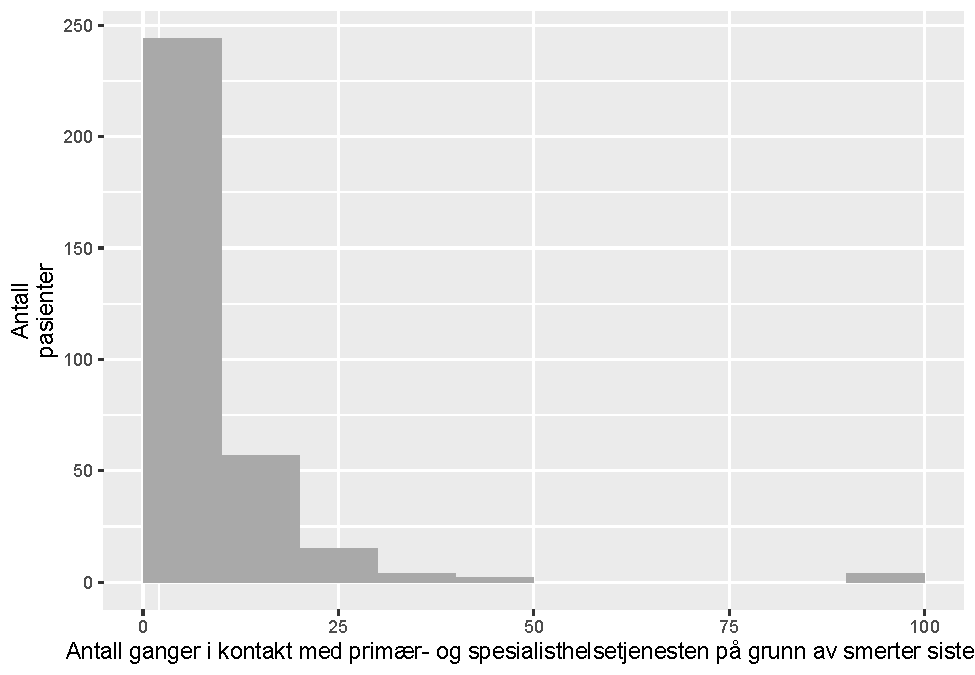
\includegraphics{lokalEpromNy_files/figure-latex/kontaktfig-1.pdf}

Figur @ref(fig:kontaktfig) viser oversikten over hvor mange ganger
pasientene har vært i kontakt med primær- og spesialisthelsetjenesten på
grunn av smerter siste år for totalt 326 pasienter.

\begin{table}

\caption{\label{tab:prsmp4}}
\centering
\begin{tabular}[t]{l|r|r}
\hline
Har tidligere opplevd belastninger som har krevd behandling av psykolog/psykiater & Antall  & Prosent\\
\hline
Nei & 263 & 60\\
\hline
Ja & 165 & 38\\
\hline
Vet ikke & 8 & 2\\
\hline
\end{tabular}
\end{table}

Tabell @ref(tab:prsmp4) viser oversikten over hvor mange av pasientene
som tidligere har opplevd belastninger som har krevd behandling av
psykolog/psykiater eller liknende for de 436 pasientene som besvarte
spørsmålet.

\begin{table}

\caption{\label{tab:prspm5}}
\centering
\begin{tabular}[t]{l|r|r}
\hline
Svar på spørsmålet: ... er det forferdelig, og jeg føler at det aldri kommer til å bli bedre & Antall  & Prosent\\
\hline
Aldri & 60 & 14\\
\hline
Nesten aldri & 45 & 10\\
\hline
Sjelden & 37 & 8\\
\hline
Av og til & 133 & 31\\
\hline
Ofte & 65 & 15\\
\hline
Nesten alltid & 59 & 14\\
\hline
Alltid & 29 & 7\\
\hline
Vet ikke & 8 & 2\\
\hline
\end{tabular}
\end{table}

Tabell @ref(tab:prspm5) viser oversikten over hvor ofte pasientene føler
`\ldots{} det er forferdelig, og jeg at det aldri kommer til å bli
bedre'. 436 pasienter besvarte spørsmålet.

\begin{table}

\caption{\label{tab:prspm6}}
\centering
\begin{tabular}[t]{l|r|r}
\hline
Svar på spørsmålet: ... føles det som om jeg ikke holder ut & Antall  & Prosent\\
\hline
Aldri & 40 & 9\\
\hline
Nesten aldri & 43 & 10\\
\hline
Sjelden & 40 & 9\\
\hline
Av og til & 127 & 29\\
\hline
Ofte & 63 & 14\\
\hline
Nesten alltid & 76 & 17\\
\hline
Alltid & 37 & 8\\
\hline
Vet ikke & 10 & 2\\
\hline
\end{tabular}
\end{table}

Tabell @ref(tab:prspm6) viser oversikten over hvor ofte pasientene føler
`\ldots{} det er som om jeg ikke holder ut'. 436 pasienter besvarte
spørsmålet.

\hypertarget{eprom-hads}{%
\section{ePROM: HADS}\label{eprom-hads}}

\begin{table}

\caption{\label{tab:hadsspm}}
\centering
\begin{tabular}[t]{l|r|r}
\hline
Grunn manglende utfylling HADS & Antall  & Prosent\\
\hline
Tidsmangel behandler & 36 & 2\\
\hline
Tidlig utskrivning & 85 & 6\\
\hline
Kritisk syk/død & 10 & 1\\
\hline
Pasient klarer ikke & 195 & 13\\
\hline
Manglende samtykke & 139 & 9\\
\hline
Ikke besvart ePPROMS & 64 & 4\\
\hline
Annet & 499 & 34\\
\hline
\end{tabular}
\end{table}

I den valgte tidsperioden fikk tilsammen 1464 pasienter av totalt 2611
tilsendt ePROM-skjema for HADS. Av de som fikk tilsendt skjema var det
435 pasienter som sendte inn en besvarelse. Dette gir en svarandel på
0.3. Tabell @ref(tab:hadsspm) gir en oversikt over registrerte årsaker
til manglende besvarelse for de 1029 som ikke har svart.

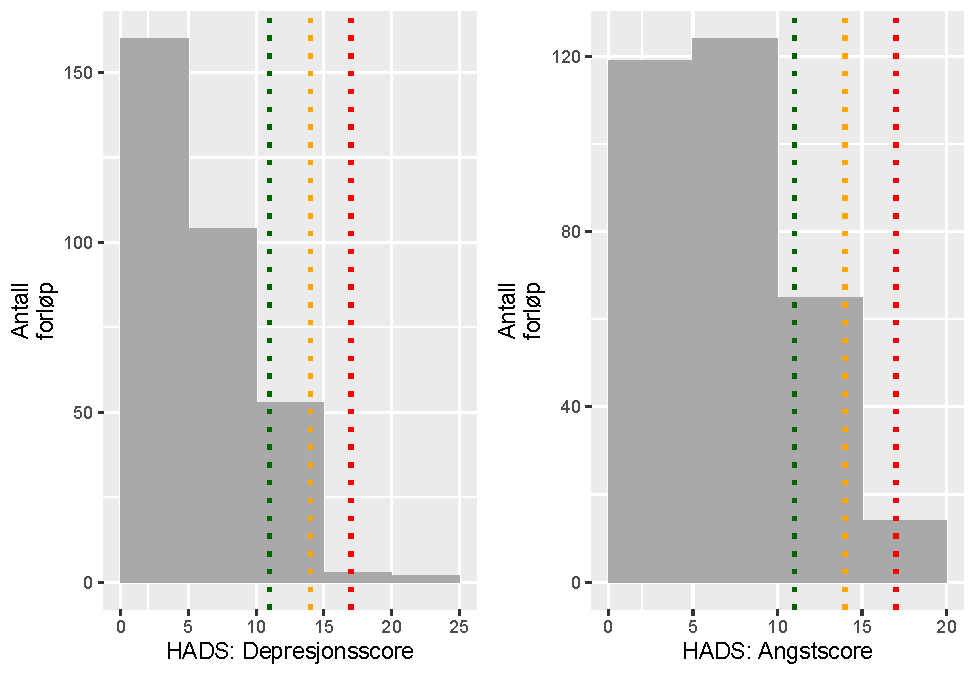
\includegraphics{lokalEpromNy_files/figure-latex/hadsfig-1.pdf}

Figur @ref(fig:hadsfig) viser viser hvordan de 435 aktuelle forløpene
fordeles på depresjonsscore og angstscore i HADS. Poengscorene vurderes
som følger: lavere enn den grønne linjen viser ingen tegn til symptomer,
mellom den grønne og den gule linjen viser milde symptomer, mellom den
gule og den røde linjen viser moderate symptomer, mens over den røde
viser alvorlig symptomer.

\hypertarget{eprom-eval}{%
\subsection{ePROM: Eval}\label{eprom-eval}}

\begin{table}

\caption{\label{tab:evalspmtab}}
\centering
\begin{tabular}[t]{l|r|r}
\hline
Grunn manglende utfylling Eval & Antall  & Prosent\\
\hline
Tidsmangel behandler & 39 & 3\\
\hline
Tidlig utskrivning & 93 & 6\\
\hline
Kritisk syk/død & 11 & 1\\
\hline
Pasient klarer ikke & 198 & 14\\
\hline
Manglende samtykke & 139 & 10\\
\hline
Ikke tilstrekkelig antall tilsyn & 19 & 1\\
\hline
Ikke besvart ePPROMS & 65 & 4\\
\hline
Annet & 516 & 35\\
\hline
\end{tabular}
\end{table}

I den valgte tidsperioden fikk tilsammen 1461 pasienter av totalt 2611
tilsendt ePROM-skjema for Eval. Av de som fikk tilsendt skjema var det
380 pasienter som sendte inn en besvarelse. Dette gir en svarandel på
0.26. Tabell @ref(tab:evalspmtab) gir en oversikt over registrerte
årsaker til manglende besvarelse for de 1081 som ikke har svart.

På spørsmålet `Husker du at du nylig har vært i kontakt med og fått
behandling av sykehusets smerteteam?' var det 10 pasienter som svarte ja
og 0 pasienter som svarte nei.

\begin{table}

\caption{\label{tab:evalspm1}}
\centering
\begin{tabular}[t]{l|r|r}
\hline
Siden oppstart av behandling fra Smerteteamet, er min smertetilstand blitt & Antall  & Prosent\\
\hline
Mye bedre & 168 & 11\\
\hline
Bedre & 114 & 8\\
\hline
Litt bedre & 54 & 4\\
\hline
Uendret & 27 & 2\\
\hline
Litt verre & 7 & 0\\
\hline
Verre & 2 & 0\\
\hline
Mye verre & 4 & 0\\
\hline
Vet ikke & 4 & 0\\
\hline
\end{tabular}
\end{table}

Tabell @ref(tab:evalspm1) viser oversikten over det første spørsmålet i
Eval: `Siden oppstart av behandling fra Smerteteamet, er min
smertetilstand blitt \ldots{}'.

\begin{table}

\caption{\label{tab:evalspm2}}
\centering
\begin{tabular}[t]{l|r|r}
\hline
Siden oppstart av behandling fra Smerteteamet, er min generelle tilstand blitt & Antall  & Prosent\\
\hline
Mye bedre & 121 & 8\\
\hline
Bedre & 140 & 10\\
\hline
Litt bedre & 59 & 4\\
\hline
Uendret & 44 & 3\\
\hline
Litt verre & 5 & 0\\
\hline
Verre & 4 & 0\\
\hline
Mye verre & 1 & 0\\
\hline
Vet ikke & 6 & 0\\
\hline
\end{tabular}
\end{table}

Tabell @ref(tab:evalspm2) viser oversikten over det andre spørsmålet i
Eval: `Siden oppstart av behandling fra Smerteteamet, er min generelle
tilstand blitt \ldots{}'.

\begin{table}

\caption{\label{tab:evalspm3}}
\centering
\begin{tabular}[t]{l|r|r}
\hline
Hvor fornøyd er du med ivaretakelsen fra Smerteteamet & Antall  & Prosent\\
\hline
Ikke i det hele tatt & 6 & 0\\
\hline
I liten grad & 12 & 1\\
\hline
I noen grad & 26 & 2\\
\hline
I stor grad & 121 & 8\\
\hline
I svært stor grad & 211 & 14\\
\hline
Vet ikke & 4 & 0\\
\hline
\end{tabular}
\end{table}

Tabell @ref(tab:evalspm3) viser oversikten over det tredje spørsmålet i
Eval: `Hvor fornøyd er du med ivaretakelsen fra Smerteteamet?'.

\begin{table}

\caption{\label{tab:evalspm4}}
\centering
\begin{tabular}[t]{l|r|r}
\hline
Snakket behandlerne i smerteteamet til deg slik at du forsto dem & Antall  & Prosent\\
\hline
I noen grad & 1 & 0\\
\hline
I stor grad & 4 & 0\\
\hline
I svært stor grad & 5 & 0\\
\hline
\end{tabular}
\end{table}

Tabell @ref(tab:evalspm4) viser oversikten over det fjerde spørsmålet i
Eval: `Snakket behandlerne i smerteteamet til deg slik at du forsto
dem?'.

\begin{table}

\caption{\label{tab:evalspm5}}
\centering
\begin{tabular}[t]{l|r|r}
\hline
Har du tillit til smerteteamets faglige dyktighet & Antall  & Prosent\\
\hline
I liten grad & 1 & 0\\
\hline
I noen grad & 2 & 0\\
\hline
I stor grad & 3 & 0\\
\hline
I svært stor grad & 4 & 0\\
\hline
\end{tabular}
\end{table}

Tabell @ref(tab:evalspm5) viser oversikten over det femte spørsmålet i
Eval: `Har du tillit til smerteteamets faglige dyktighet?'.

\begin{table}

\caption{\label{tab:evalspm6}}
\centering
\begin{tabular}[t]{l|r|r}
\hline
Fikk du tilstrekkelig informasjon og forklaring om din smertetilstand & Antall  & Prosent\\
\hline
I noen grad & 3 & 0\\
\hline
I stor grad & 5 & 0\\
\hline
I svært stor grad & 1 & 0\\
\hline
Vet ikke & 1 & 0\\
\hline
\end{tabular}
\end{table}

Tabell @ref(tab:evalspm6) viser oversikten over det sjette spørsmålet i
Eval: `Fikk du tilstrekkelig informasjon og forklaring om din
smertetilstand?'.

\begin{table}

\caption{\label{tab:evalspm7}}
\centering
\begin{tabular}[t]{l|r|r}
\hline
Opplevde du at smertebehandlingen var tilpasset din situasjon & Antall  & Prosent\\
\hline
I noen grad & 3 & 0\\
\hline
I stor grad & 3 & 0\\
\hline
I svært stor grad & 3 & 0\\
\hline
Vet ikke & 1 & 0\\
\hline
\end{tabular}
\end{table}

Tabell @ref(tab:evalspm7) viser oversikten over det syvende spørsmålet i
Eval: `Opplevde du at smertebehandlingen var tilpasset din situasjon?'.

\begin{table}

\caption{\label{tab:evalspm8}}
\centering
\begin{tabular}[t]{l|r|r}
\hline
Var du involvert i avgjørelser som angikk din smertebehandling & Antall  & Prosent\\
\hline
Ikke i det hele tatt & 1 & 0\\
\hline
I noen grad & 2 & 0\\
\hline
I stor grad & 5 & 0\\
\hline
I svært stor grad & 2 & 0\\
\hline
\end{tabular}
\end{table}

Tabell @ref(tab:evalspm8) viser oversikten over det åttende spørsmålet i
Eval: `Var du involvert i avgjørelser som angikk din smertebehandling?'.

\begin{table}

\caption{\label{tab:evalspm9}}
\centering
\begin{tabular}[t]{l|r|r}
\hline
Opplevde du at smerteteamets arbeid var godt organisert & Antall  & Prosent\\
\hline
I liten grad & 1 & 0\\
\hline
I noen grad & 2 & 0\\
\hline
I stor grad & 4 & 0\\
\hline
I svært stor grad & 3 & 0\\
\hline
\end{tabular}
\end{table}

Tabell @ref(tab:evalspm9) viser oversikten over det niende spørsmålet i
Eval: `Opplevde du at smerteteamets arbeid var godt organisert?'.

\begin{table}

\caption{\label{tab:evalspm10}}
\centering
\begin{tabular}[t]{l|r|r}
\hline
Var hjelpen og behandlingen du fikk av smerteteamet, alt i alt, tilfredsstillende & Antall  & Prosent\\
\hline
I noen grad & 4 & 0\\
\hline
I stor grad & 3 & 0\\
\hline
I svært stor grad & 3 & 0\\
\hline
\end{tabular}
\end{table}

Tabell @ref(tab:evalspm10) viser oversikten over det tiende spørsmålet i
Eval: `Var hjelpen og behandlingen du fikk av smerteteamet, alt i alt,
tilfredsstillende?'.

\begin{table}

\caption{\label{tab:evalspm11}}
\centering
\begin{tabular}[t]{l|r|r}
\hline
Mener du at du på noen måte ble feilbehandlet av smerteteamet? & Antall  & Prosent\\
\hline
Ikke i det hele tatt & 6 & 0\\
\hline
I liten grad & 1 & 0\\
\hline
I noen grad & 3 & 0\\
\hline
\end{tabular}
\end{table}

Tabell @ref(tab:evalspm11) viser oversikten over det ellevte spørsmålet
i Eval: `Mener du at du på noen måte ble feilbehandlet av smerteteamet
(etter det du selv kan bedømme)?'.

\hypertarget{eprom-opioid}{%
\subsection{ePROM: Opioid}\label{eprom-opioid}}

\begin{table}

\caption{\label{tab:opiospmtab}}
\centering
\begin{tabular}[t]{l|r|r}
\hline
Grunn manglende utfylling Opioid & Antall  & Prosent\\
\hline
Kritisk syk/død & 1 & 0\\
\hline
Pasient klarer ikke & 8 & 3\\
\hline
Manglende samtykke & 107 & 44\\
\hline
Ikke besvart ePPROMS & 48 & 20\\
\hline
Annet & 18 & 7\\
\hline
\end{tabular}
\end{table}

I den valgte tidsperioden fikk tilsammen 245 pasienter av totalt 2611
tilsendt ePROM-skjema for Opioid. Av de som fikk tilsendt skjema var det
63 pasienter som sendte inn en besvarelse. Dette gir en svarandel på
0.26. Tabell @ref(tab:opiospmtab) gir en oversikt over registrerte
årsaker til manglende besvarelse for de 182 som ikke har svart.

På spørsmål om pasienten var skrevet ut av sykehus (ved besvarelse) var
det 54 pasienter som svarte ja, mens 9 pasienter svarte nei. Av de som
svarte ja, var det 48 som hadde brukt sterke smertestillende
medikamenter etter at de ble skrevet ut fra sykehuset, mens 6 svarte nei
på dette.

\begin{table}

\caption{\label{tab:medtab}}
\centering
\begin{tabular}[t]{l|r}
\hline
  & Antall ja\\
\hline
DolcontinMalfin & 14\\
\hline
FentanylplDurogesicpl & 7\\
\hline
Metadon & 1\\
\hline
Morfin & 15\\
\hline
Norspanplaster & 4\\
\hline
OxynormOxykodon & 21\\
\hline
OxyxontinReltebon & 9\\
\hline
Palexia & 1\\
\hline
PalladonHydromorfon & 0\\
\hline
Paralginforte & 4\\
\hline
Buprenorfin & 0\\
\hline
Targiniq & 3\\
\hline
Tramadolvarianter & 6\\
\hline
Andre & 4\\
\hline
Usikker & 3\\
\hline
\end{tabular}
\end{table}

\begin{table}

\caption{\label{tab:medforts}}
\centering
\begin{tabular}[t]{l|r|r}
\hline
Bruker du fortsatt noen av disse medikamentene? & Antall  & Prosent\\
\hline
Nei & 11 & 4\\
\hline
Ja, i samme dosering & 17 & 7\\
\hline
Ja, i lavere dosering & 20 & 8\\
\hline
\end{tabular}
\end{table}

Tabell @ref(tab:medtab) viser en oversikt over hvilke medikamenter som
har blitt brukt av pasientene etter utskrivelse, mens tabell
@ref(tab:medforts) viser hvor mange som fortsatt bruker disse
medikamentene når de besvarer spørsmålet.

\begin{table}

\caption{\label{tab:infonedtab}}
\centering
\begin{tabular}[t]{l|r|r}
\hline
Fikk du informasjon om nedtrapping av sterke smertestillende medikamenter? & Antall  & Prosent\\
\hline
Nei & 11 & 4\\
\hline
Ja & 37 & 15\\
\hline
\end{tabular}
\end{table}

\begin{table}

\caption{\label{tab:nedtrhvem}}
\centering
\begin{tabular}[t]{l|r|r}
\hline
Av hvem fikk du informasjon om nedtrapping av sterke smertestillende medikamenter? & Antall  & Prosent\\
\hline
Smerteteam & 19 & 8\\
\hline
Annet helsepersonell & 7 & 3\\
\hline
Begge & 10 & 4\\
\hline
Vet ikke & 1 & 0\\
\hline
\end{tabular}
\end{table}

Tabell @ref(tab:infonedtab) viser om pasienten har fått informasjon om
nedtrapping av sterke smertestillende medikamenter, mens tabell
@ref(tab:nedtrhvem) viser hvem som har formidlet informasjonen.

\begin{table}

\caption{\label{tab:nedrfulgtplan}}
\centering
\begin{tabular}[t]{l|r|r}
\hline
Klarte du å følge anbefalingene for bruk og nedtrapping av medikamentene? & Antall  & Prosent\\
\hline
Ja & 21 & 9\\
\hline
Nei, lenger enn anbefalt & 11 & 4\\
\hline
Nei, har ikke kunnet trappe ned & 2 & 1\\
\hline
Ja, raskere & 3 & 1\\
\hline
\end{tabular}
\end{table}

Det er 26 pasienter som har fått muntlig informasjon om nedtrapping,
mens 48 pasienter svarte at de ikke har fått det. Samtidig svarer 24
pasienter at de har fått skriftlig nedtrappingsplan, mens 48 svarer nei
på dette. I tillegg svarer 8 pasienter at de fikk utdelt infobrosjyre om
nedtrapping, mens 48 svarer at de ikke fikk den utdelt.

Tabell @ref(tab:nedrfulgtplan) viser hva pasientene har svart på om de
klarte å følge anbefalingene for bruk og nedtrapping av medikamentene.

\begin{table}

\caption{\label{tab:abstietter}}
\centering
\begin{tabular}[t]{l|r|r}
\hline
Opplevde du plagsomme abstinenssymptomer etter utskrivelse? & Antall  & Prosent\\
\hline
Nei & 30 & 12\\
\hline
Ja & 9 & 4\\
\hline
Usikker & 9 & 4\\
\hline
\end{tabular}
\end{table}

\begin{table}

\caption{\label{tab:abstiforstod}}
\centering
\begin{tabular}[t]{l|r|r}
\hline
Forstod du at det var abstinenssymptomer? & Antall  & Prosent\\
\hline
Ja & 8 & 3\\
\hline
Usikker & 1 & 0\\
\hline
\end{tabular}
\end{table}

\begin{table}

\caption{\label{tab:abstilosn}}
\centering
\begin{tabular}[t]{l|r|r}
\hline
Visste du hva du kunne gjøre med problemet? & Antall  & Prosent\\
\hline
Nei & 2 & 1\\
\hline
Ja & 6 & 2\\
\hline
Usikker & 1 & 0\\
\hline
\end{tabular}
\end{table}

Tabell @ref(tab:abstietter) viser en oversikt over om pasienten har
opplevd abstinenssymptomer (svetting/frysing, uro, smerter, diaré,
rennende nese) etter utskrivelse, mens tabell @ref(tab:abstiforstod)
viser om pasienten forstod at det var abstinenssymptomer eller ikke.
Tabell @ref(abstilosn) viser om pasienten visste hva den kunne gjøre med
problemet.

\begin{table}

\caption{\label{tab:tretth}}
\centering
\begin{tabular}[t]{l|r|r}
\hline
Opplevde du plagsom tretthet eller følelse av å være medikamentpåvirket etter at du ble skrevet ut fra sykehuset? & Antall  & Prosent\\
\hline
Nei & 36 & 15\\
\hline
Ja & 12 & 5\\
\hline
\end{tabular}
\end{table}

\begin{table}

\caption{\label{tab:trettvisste}}
\centering
\begin{tabular}[t]{l|r|r}
\hline
Visste du hva du kunne gjøre med problemet? & Antall  & Prosent\\
\hline
Nei & 3 & 1\\
\hline
Ja & 3 & 1\\
\hline
Vet ikke & 6 & 2\\
\hline
\end{tabular}
\end{table}

Tabell @ref(tab:tretth) viser en oversikt over spørsmålet ``Opplevde du
plagsom tretthet eller følelse av å være medikamentpåvirket etter at du
ble skrevet ut fra sykehuset?'', mens tabell @ref(tab:trettvisste) viser
om pasienten visste hva å gjøre hvis den opplevde dette.

\begin{table}

\caption{\label{tab:sterkbil}}
\centering
\begin{tabular}[t]{l|r|r}
\hline
Fikk du informasjon om sterke smertestillende medikamenter og bilkjøring? & Antall  & Prosent\\
\hline
Nei & 12 & 5\\
\hline
Ja & 32 & 13\\
\hline
Ikke aktuelt & 4 & 2\\
\hline
\end{tabular}
\end{table}

\begin{table}

\caption{\label{tab:hveminfobil}}
\centering
\begin{tabular}[t]{l|r|r}
\hline
Av hvem fikk du informasjon om sterke smertestillende medikamenter og bilkjøring? & Antall  & Prosent\\
\hline
Smerteteam & 6 & 2\\
\hline
Annet helsepersonell & 6 & 2\\
\hline
Begge & 19 & 8\\
\hline
Vet ikke & 1 & 0\\
\hline
\end{tabular}
\end{table}

\begin{table}

\caption{\label{tab:bil}}
\centering
\begin{tabular}[t]{l|r|r}
\hline
Visste du hvor du kunne henvende deg ved spørsmål om bruk av de smertestillende medikamentene? & Antall  & Prosent\\
\hline
Nei & 12 & 5\\
\hline
Ja & 33 & 13\\
\hline
Usikker & 3 & 1\\
\hline
\end{tabular}
\end{table}

Tabell @ref(tab:sterkbil) viser en oversikt over spørsmålet ``Fikk du
informasjon om sterke smertestillende medikamenter og bilkjøring?'',
mens tabell @ref(tab:hveminfobil) viser hvem som formidlet denne
informasjonen.

Det er 28 pasienter som har fått muntlig informasjon om medikamenter og
bilkjøring, mens 48 pasienter har svart at de ikke har fått det.
Samtidig svarer 6 pasienter at de har fått skriftlig info om
medikamenter og bilkjøring, mens 48 svarer nei på dette. I tillegg
svarer 11 pasienter at de har fått utdelt infobrosjyre «Sterke
smertestillende -- informasjon om kortvarig bruk og nedtrapping», mens
48 svarer at de ikke fikk den utdelt.

\end{document}
